\documentclass{article}
\usepackage{graphicx} % Required for inserting images
\usepackage[english]{babel}
\usepackage{amsmath}
\usepackage{amsthm}
\usepackage{amssymb}
\usepackage[margin=.75in]{geometry}
\usepackage{hyperref}
\usepackage{amsfonts}
\usepackage{mathrsfs}
\usepackage[version=4]{mhchem}
\usepackage{bigints}
\usepackage{caption}
\usepackage{xpatch}
\usepackage{xr}
\usepackage{enumitem}
\usepackage{subcaption}
\usepackage[american,siunitx]{circuitikz}
\usepackage{tikz}
\usetikzlibrary{arrows.meta, positioning}
\usetikzlibrary{patterns, angles, quotes, calc}
\setlength{\parindent}{0pt}

\title{Landau and Lifshitz Mechanics Notes}
\author{Kyle Wang}
\date{November 2026}

\newcommand{\pd}[2]{\frac{\partial #1}{\partial #2}}
\newcommand{\od}[2]{\frac{d #1}{d #2}}
\newcommand{\twen}{\hspace{20pt}}
\newcommand{\lagr}{\mathscr{L}}

\newtheorem{theorem}{Theorem}[section]
\newtheorem{lemma}[theorem]{Lemma}
\newtheorem{corollary}[theorem]{Corollary}
\theoremstyle{definition}
\newtheorem{definition}[theorem]{Definition}
\newtheorem{example}[theorem]{Example}
\newtheorem{problem}{Problem}[section]
\theoremstyle{remark}
\newtheorem*{work}{Work}

\begin{document}

\maketitle

\section{Equations of Motion}
To define the position of $N$ particles in space, we need to specify $N$ radius vectors and hence $3N$ coordinates. The number of independent quantities to uniquely determine the position of a system are known as the \emph{degrees of freedom}. These coordinates need not be Cartesian, any $s$ quantities $q_1,q_2,\ldots, q_s$ that uniquely define the position of a system with $s$ degrees of freedom are the generalized coordinates of the system and the derivatives are the generalized velocities. However, since the velocities can be anything given a specific set of generalized coordinates, we need to specify these velocities in order to uniquely determine the accelerations and \emph{state} of a system.
\subsection{Principle of Least Action}
The law that governs mechanical systems is the \emph{principle of least action} (otherwise known as Hamilton's principle) where every system is characterized by a function known a the \emph{Lagrangian} defined as$\lagr(q_1,q_2,\ldots, q_s,\dot q_1,\dot q_2, \ldots, \dot q_s,t)$ or more concisely, $\lagr(q,\dot q,t)$. At the times $t=t_1$ and $t=t_2$, let us define the system to occupy the coordinates $q^{(1)}$ and $q^{(2)}$. Then we require that the system moves in a way such that the integral 
\begin{equation}
    S=\int^{t_2}_{t_1} \lagr (q,\dot q,t)dt
\end{equation}
is minimized. This quantity is known as the \emph{action}. Let us minimize the integral when only given one degree of freedom. Let $q=q(t)$ be the function for which $S$ is at its minimum. When we choose a path $q(t)+\delta q(t)$, we add a \emph{variation} (which is more generally an idea from the calculus of variations). This variation $\delta q(t)$ on $q(t)$ must be zero at times $t_1$ and $t_2$ so that the two paths start and end at the same location. Then we have that the change in action of this new varied path to be 
\begin{equation*}
    \delta S =\int^{t_2}_{t_1}\lagr (q+ \delta q, \dot q+\delta \dot q, t)dt - \int^{t_2}_{t_1} \lagr (q,\dot q,t)dt
\end{equation*}
If we recall the properties of the minimum, we recall that the derivative is zero there and so any first order change yields approximately zero change in the function. Therefore $\delta S =0$. We now have that 
\begin{equation*}
    \begin{split}
        \delta S &= \delta \int^{t_2}_{t_1} \lagr (q,\dot q,t)dt \\
        &= \int^{t_2}_{t_1} \left( \pd{\lagr}{q} \delta q + \pd{\lagr}{\dot q} \delta \dot q \right) dt = 0
    \end{split}
\end{equation*}
Since $\delta \dot q = \od{ \delta q}{t}$, we can integrate by parts (and ``move" the derivative) on the second to get 
\begin{equation*}
    \delta S = \pd{\lagr}{\dot q} \delta q \Bigg|^{t_2}_{t_1} + \int^{t_2}_{t_1} \left( \pd{\lagr}{q} - \od{}{t} \pd{\lagr }{\dot q} \right) \delta q dt = 0
\end{equation*}
Since $\delta q(t_1)=\delta q(t_2)=0$, the first term disappears and in order for the resulting integral to always be zero, we must have that 
\begin{equation}
    \od{}{t} \pd{\lagr}{\dot q} - \pd{\lagr }{q} =0
\end{equation}
which are known as the \emph{Euler-Lagrange Equations}. For a system with $n$ degrees of freedom, we use instead 
\begin{equation}
    \od{}{t} \pd{\lagr}{\dot q_i} - \pd{\lagr }{q_i} =0 \twen i\in \{ 1,2,\ldots,n\}
\end{equation}
When we use these equations, we get the equations of motions which dictates the particle's acceleration, position, and velocity. We also need initial conditions to use to uniquely determine the path the system takes. \\\\
If we consider a mechanical system with two parts in a closed system such that they have the Lagrangians $\lagr_A$ and $\lagr_B$ for $A$ and $B$ respectively. In the limit when the distance between the parts becomes large enough such that the interaction between them are negligible, we have 
\begin{equation}
    \lim \lagr = \lagr_A + \lagr_B \label{eq:addLagr}
\end{equation}
The additivity of the Lagrangian implies that the equations of motions of either cannot involve quantities relating to the other. We can also multiply the Lagrangian by any arbitrary constant without affecting the equations of motion. This correlates with a change of units. However, we trivially note that all Lagrangians of a system must be multiplied by the same arbitrary constant by \eqref{eq:addLagr}. \\\\
The final remark is that the Lagrangian isn't unique. If we consider Lagrangians $\lagr ' $ and $\lagr$, that differ by 
\begin{equation}
    \lagr ' = \lagr + \od{}{t}f(q,t)
\end{equation}
The actions we get are 
\begin{equation*}
    S' = \int^{t_2}_{t_1} \lagr ' dt = \int^{t_2}_{t_1} \lagr dt + \int^{t_2}_{t_1} \od{f}{t} dt = S + f(q^{(2)},t_2) -f(q^{(1)},t_1)
\end{equation*}
which when varied, we get that $\delta S' =\delta S =0$. This effectively means the Lagrangian is the same within different frames of reference or reference potentials and we can safely discard these $f(q,t)$ terms classically (although quantum mechanically, they are much more important).
\subsection{Lagrangian of a Free Particle}
We can always find a frame of reference such that space and time are \emph{homogeneous}. This is known as an \emph{inertial frame}. If space and time were inhomogeneous, then that means different frames of references and points in time yield mechanically different systems, even if there were no other bodies. Because of this homogeneity of space and time, the Lagrangian cannot explicitly be a function of the radius vector $\vec{r}$ of the particle or $t$. Therefore $\lagr$ must be a function of $\vec v$ but once again, the isotropy of space means it can only be a function of its magnitude $v^2$. Since the Lagrangian is independent of $\vec r$, the Euler Lagrange equation turns into 
\begin{equation*}
    \od{}{t} \pd{\lagr}{\vec v} =0
\end{equation*}
and therefore 
\begin{equation*}
    \begin{split}
        \pd{\lagr}{\vec v} &= C \\
        \pd{\lagr(v^2)}{\vec v} = \pd{\lagr(v^2)}{(v^2)}& \pd{(v^2)}{\vec v} = 2\pd{\lagr(v^2)}{(v^2)}\vec v =C
    \end{split}
\end{equation*}
and so $\vec{v}$ is a constant. Note Landau uses $\pd{}{\vec v} = \nabla_{\vec{v}}$. Thus any free motion takes place with a velocity that is constant in magnitude and direction. This is the law of inertia. If there is another inertial frame moving uniformly relative to the other inertial frame, then the system is equivalent mechanically. In fact there are an infinite number of equivalent reference frames. This is known as \emph{Galileo's relativity principle}. It effectively states that physics does not have an absolute preferred reference frame. If $\vec{r} $ and $\vec{r}'$ describe the point in two different frames $K$ and $K'$ and one moves with a velocity $\vec V$ relative to the other, then they are related by 
\begin{equation*}
    \vec r=\vec r'+\vec Vt
\end{equation*}
and $t=t'$. \\\\
Let us now determine the Lagrangian of a free particle relative to an inertial frame. If we have another inertial frame $K'$ moving such that $\vec v'=\vec v+\vec \varepsilon$, the Lagrangians must be the same in both frames by Galilean relativity and so $\lagr ' = \lagr(v'^2) =\lagr(v^2+2\vec v\cdot \vec \varepsilon + \varepsilon^2)$ and ignoring higher orders of $\varepsilon$ and Taylor expanding around $ v^2$, we get
\begin{equation*}
    \lagr (v'^2) = \lagr(v^2) + \pd{\lagr}{v^2} 2\vec v\cdot \vec \varepsilon
\end{equation*}
The second term on the right hand side is a total time derivative if and only if $\pd{\lagr}{v^2}$ is independent of $\vec v$. That means we can represent it with a constant $c$ and so turn that term into $\od{}{t}(2c\vec r \cdot \vec \varepsilon)$. We require this because we want that term to simply be a result of the frame of reference and not anything mechanically different with the system. Therefore, we can integrate to get 
\begin{equation*}
    \pd{\lagr}{v^2} = c \Rightarrow \lagr = cv^2
\end{equation*}
and if we let this constant $c=\frac{1}{2}m$, we see that the Lagrangian of a free particle takes the form 
\begin{equation}
    \lagr = \frac{1}{2}mv^2
\end{equation}
We can see this hold up for a non-infinitessimal relative velocity when two frames $K$ and $K'$ move at $\vec V$ relative to each other. Therefore 
\begin{equation*}
    \begin{split}
        \lagr ' &= \frac{1}{2}mv'^2 = \frac{1}{2}m(\vec v+\vec V)^2 \\&= \frac{1}{2}mv^2 + m\vec v\cdot \vec V + \frac{1}{2}mV^2 \\
        &= \lagr + \od{}{t}\left(m\vec r \cdot \vec V + \frac{1}{2} mV^2\right)
    \end{split}
\end{equation*}
and we can once again discard the time derivative term. $m$ is known as the mass of the particle. Using the additive property of Lagrangians, a system of non interacting particles has the Lagrangian 
\begin{equation*}
    \lagr = \sum_i \frac{1}{2}m_iv_i^2
\end{equation*}
We can also see using the definition of the action, that mass can't be negative. The integral 
\begin{equation*}
    S= \frac{1}{2}\int^{t_2}_{t_1}mv^2dt
\end{equation*}
can never reach a minimum if mass is negative since it would yield arbitrarily large negative values.\\\\
Severely abusing notation like an alcoholic father, we get 
\begin{equation*}
    v^2 = \left( \od{l}{t}\right)^2 = \frac{(dl)^2}{(dt)^2}
\end{equation*}
and so the Lagrangian under different coordinates are as follows 
\begin{equation*}
    \begin{split}
        \lagr_{\text{Cart.}} & = \frac{1}{2}m(\dot x^2+\dot y^2+\dot z^2) \\
        \lagr_{\text{Cyl.}}&= \frac{1}{2}m(\dot r^2 + r^2 \dot \phi^2 + \dot z^2) \\
        \lagr_{\text{Sph.}}&=\frac{1}{2}m(\dot r^2+r\dot \theta^2 + r^2 \dot \phi ^2\sin^2 \theta)
    \end{split}
\end{equation*}
\subsection{Lagrangian for a System of Particles}
Consider a system of particles that interact with each other but no other bodies. This is deemed a \emph{closed} system. It turns out the interaction can be modeled by the Lagrangian by adding a function of the coordinates $-U$ such that 
\begin{equation}
    \lagr = \sum_i \frac{1}{2}m_i v_i^2 -U(\vec r_1,\vec r_2,\ldots)
\end{equation}
The first term is deemed the kinetic energy $T$ and the second term is the potential energy $U$ of the system. This book does not contain relativistic mechanics and so as a result of Galilean relativity, changes in position of each of the particles propagate instantly because otherwise, different reference frames would view the speed of propagation to be different.\\\\
If we know the Lagrangian of a system of particles, then we get via the Euler-Lagrange equations
\begin{equation*}
    \begin{split}
        \od{}{t}\pd{\lagr}{\vec v_i} &=\pd {\lagr}{\vec r_i} \\
        m_a \od{\vec v_i}{t} &=-\pd{U}{\vec r_i}
    \end{split}
\end{equation*}
where we define the quantity $\vec F$ to be the \emph{force} on the $i^{th}$ particle
\begin{equation*}
    \vec F= -\pd{U}{\vec r_i}
\end{equation*}
The potential is only defined to a constant which varies depending on reference. The canonical reference is zero as the distance between two interacting particles goes to infinity.\\\\
Suppose we want to work with some generalized set of coordinates $q_i$. Then let us define a smooth map $f:\mathbb{R}^s \to \mathbb{R}^s$ such that 
\begin{equation*}
    \vec x_i = f_i(q_1,q_2,\ldots,q_s) \twen \dot{ \vec {x}}_i= \sum_k \pd{f}{q_k}\od{\dot q_k}{t} 
\end{equation*}
Substituting this into our closed system Lagrangian, we get 
\begin{equation*}
    \begin{split}
        \lagr &= \sum_i\frac{1}{2} m_i \left( \sum_j\pd{f_i}{q_j}\dot q_j \right) \left( \sum_k\pd{f_i}{q_k}\dot q_k \right) \\
        &= \sum_{j,k} \frac{1}{2}\left( \sum_i m_i \pd{f_i}{q_j}\cdot \pd{f_i}{q_k} \right)\dot q_j \dot q_k
    \end{split}
\end{equation*}
Let us now define 
\begin{equation*}
    a_{jk}(q) := \sum_i m_i \pd{f_i}{q_j}\cdot \pd{f_i}{q_k}
\end{equation*}
It is worth remembering that $f_i$ yields a vector quantity and the dot product commutes. Therefore the final generalized Lagrangian is 
\begin{equation}
    \lagr = \frac{1}{2}\sum_{j,k}a_{jk}(q) \dot q_j \dot q_k -U(q)
\end{equation} 
Let us now suppose a system $A$ isn't closed and interacts with another system $B$. Then assuming the $A+B$ system is closed, we can describe their combined Lagrangian as 
\begin{equation*}
    \lagr_{A+B} = T_A(q_A,\dot q_A) + T_B(q_B,\dot q_B) -U(q_A,q_B)
\end{equation*}
If we substitute $q_B$ for some $q_B(t)$ and so the Lagrangian of system $A$ is 
\begin{equation}
    \lagr_A =T_A(q_A,\dot q_A) - U(q_A,q_B(t))
\end{equation}
When a single particle moves through some external field, the Lagrangian is 
\begin{equation*}
    \lagr = \frac{1}{2}mv^2-U(\vec r,t) 
\end{equation*}
and so hence the equation of motion is 
\begin{equation*}
    m\dot{\vec{v}} =-\pd{U}{\vec r}
\end{equation*}
A field that acts on the particle with the same force at every point is deemed \emph{uniform}. We can find $U$ by integrating such that 
\begin{equation*}
    U = -\int^{\vec{r}_2}_{\vec r_1} \vec F \cdot d\vec r
\end{equation*}
\subsection{Problems}
\begin{problem}
Find the Lagrangian of the double pendulum (Figure \ref{fig:double_pendulum}).
\begin{figure}[htbp]
  \centering
  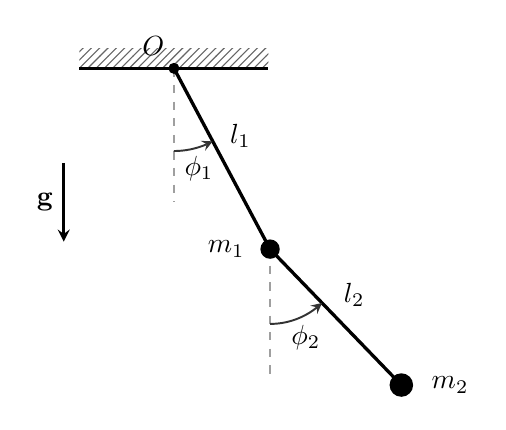
\begin{tikzpicture}[
      >=stealth,
      rod/.style={line width=1.2pt, black},
      dashedref/.style={dashed, gray!75, line width=0.7pt},
      mass/.style={circle, fill=black, inner sep=0pt},
      anglemark/.style={draw=black!80, ->, line width=0.7pt}
  ]

  % --- Parameters ---
  \def\lone{2.6}       % Length l_1
  \def\ltwo{2.4}       % Length l_2
  \def\phione{28}      % Angle phi_1 (degrees CCW from downward vertical)
  \def\phitwo{44}      % Angle phi_2 (degrees CCW from downward vertical)

  % --- Coordinates ---
  \coordinate (O)  at (0,0);
  \coordinate (V0) at (0, -1.7); % Reference vertical below O
  \coordinate (M1) at ($(O) + (\phione - 90:\lone)$);
  \coordinate (V1) at ($(M1) + (0, -1.6)$); % Reference vertical below m_1
  \coordinate (M2) at ($(M1) + (\phitwo - 90:\ltwo)$);

  % --- Support / Ceiling ---
  \fill[pattern=north east lines, pattern color=black!60] (-1.2, 0) rectangle (1.2, 0.25);
  \draw[line width=1pt] (-1.2, 0) -- (1.2, 0);

  % --- Vertical Reference Lines ---
  \draw[dashedref] (O)  -- (V0);
  \draw[dashedref] (M1) -- (V1);

  % --- Rods ---
  \draw[rod] (O)  -- node[above right, midway, xshift=-1pt] {$l_1$} (M1);
  \draw[rod] (M1) -- node[above right, midway, xshift=-1pt] {$l_2$} (M2);

  % --- Angle Arcs ---
  \pic[anglemark, "$\phi_1$", angle radius=1.05cm, angle eccentricity=1.25] {angle = V0--O--M1};
  \pic[anglemark, "$\phi_2$", angle radius=0.95cm, angle eccentricity=1.28] {angle = V1--M1--M2};

  % --- Pivot and Masses ---
  \fill[black] (O) circle (2pt) node[above left, yshift=1pt] {$O$};
  \node[mass, minimum size=7pt, label={[left, xshift=-2pt]left:$m_1$}] at (M1) {};
  \node[mass, minimum size=8.5pt, label={[right, xshift=3pt]right:$m_2$}] at (M2) {};

  % --- Gravity Vector ---
  \draw[->, line width=0.9pt] (-1.4, -1.2) -- (-1.4, -2.2) node[midway, left] {$\mathbf{g}$};

  \end{tikzpicture}
  \caption{Coplanar double pendulum with generalized coordinates $\phi_1$ and $\phi_2$ measured from the downward vertical.}
  \label{fig:double_pendulum}
\end{figure}
\end{problem}
\begin{work}
    We can express the coordinates of mass 1 as 
    \begin{equation*}
        \begin{split}
            x_1 &= l_1 \sin \phi_1 \Rightarrow \dot x =l_1 \dot \phi_1 \cos \phi_1 \\
            y_1 &= l_1 \cos \phi_1 \Rightarrow \dot y = -l_1 \dot \phi_1 \sin \phi_1
        \end{split}
    \end{equation*}
    Therefore $\dot x^2_1 +\dot y^2_1 = l_1^2 \dot \phi_1^2$. The coordinates of mass 2 are a little bit harder. We have that 
    \begin{equation*}
        \begin{split}
            x_2 &= l_1 \sin \phi_1 +l_2 \sin\phi_2 \Rightarrow \dot x_2 = l_1\dot \phi_1\cos \phi_1 +l_2 \dot \phi_2 \cos \phi_2 \\
            y_2 &= l_1 \cos \phi_1 +l_2 \cos\phi_2 \Rightarrow \dot x_2 = -l_1\dot \phi_1\sin \phi_1 -l_2 \dot \phi_2 \sin \phi_2 \\
        \end{split}
    \end{equation*}
    and so therefore $\dot x^2_2 + \dot y_2^2 $ is equal to 
    \begin{equation*}
        \begin{split}
            \dot x^2_2 + \dot y_2^2 &= l_1^2\dot\phi_1^2 + l_2^2\dot \phi_2^2 + l_1l_2\phi_1 \phi_2 (\sin \phi_1 \sin \phi_2 + \cos \phi_1 \cos \phi_2) \\
            &=l_1^2\dot\phi_1^2 + l_2^2\dot \phi_2^2 + l_1l_2\phi_1 \phi_2 \cos(\phi_1 - \phi_2)
        \end{split}
    \end{equation*}
    The potentials of each of the masses are 
    \begin{equation*}
        \begin{split}
            V_1 &= -m_1gl_2 \cos \phi_1 \\
            V_2 &= -m_2g(l_1 \cos \phi_1 +l_2 \cos \phi_2)
        \end{split}
    \end{equation*}
    So thus the Lagrangian is 
    \begin{equation*}
        \mathscr{L} = \frac{1}{2} m_1 l_1^2 \dot \phi_1^2 + \frac{1}{2}m_2(l_1^2\dot \phi_1^2+l_2^2\dot \phi_2^2 + 2l_1l_2\dot \phi_1\dot\phi_2\cos(\phi_1-\phi_2)) + m_1gl_2\cos \phi_1 +m_2g(l_1\cos \phi_1 + l_2\cos\phi_2)
    \end{equation*}
\end{work}

\begin{problem}
Find the Lagrangian of a simple pendulum of mass $m_2$ with a mass $m_1$ at the point of support which can move on a horizontal line lying in the plane in which $m_2$ moves (Figure \ref{fig:moveablePendulum}).
    \begin{figure}
        \centering
        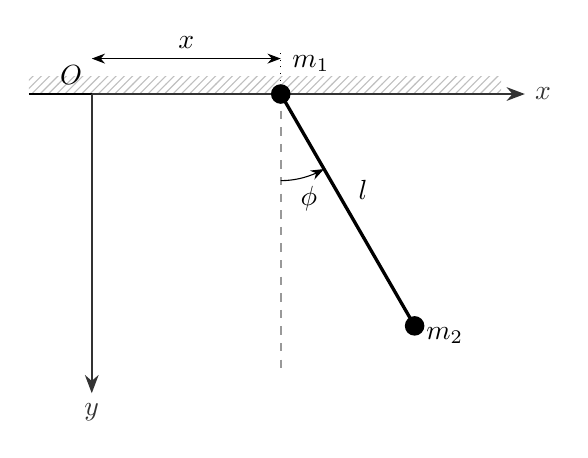
\begin{tikzpicture}[
    >=Stealth,
    mass/.style={circle, fill=black, inner sep=2.5pt},
    axis/.style={->, thick, black!80},
    dashedline/.style={dashed, gray!80, thick}]

    % Parameters for geometry
    \def\xval{2.4}      % Horizontal displacement x of m1
    \def\len{3.4}       % Length l of the pendulum
    \def\ang{30}        % Angle phi in degrees

    % Key coordinates
    \coordinate (O) at (0,0);
    \coordinate (M1) at (\xval, 0);
    \coordinate (V) at (\xval, -2.0); % Point vertically below m1 for angle arc
    \coordinate (M2) at ({\xval + \len*sin(\ang)}, {-\len*cos(\ang)});

    % Fixed horizontal track / ceiling hatch
    \fill[pattern=north east lines, pattern color=gray!50] (-0.8, 0) rectangle (5.2, 0.22);
    \draw[thick] (-0.8, 0) -- (5.2, 0);

    % Coordinate axes (x horizontal, y downward per Landau)
    \draw[axis] (O) -- (5.5, 0) node[right] {$x$};
    \draw[axis] (O) -- (0, -3.8) node[below] {$y$};
    \node[above left] at (O) {$O$};

    % Displacement x indicator
    \draw[<->, thin] (0, 0.45) -- (\xval, 0.45) node[midway, above] {$x$};
    \draw[dotted] (\xval, 0) -- (\xval, 0.55);

    % Vertical reference line through m1
    \draw[dashedline] (M1) -- (\xval, -3.5);

    % Pendulum rod of length l
    \draw[very thick] (M1) -- (M2) node[midway, above right] {$l$};

    % Angle phi
    \pic[draw, ->, "$\phi$", angle radius=1.1cm, angle eccentricity=1.25] {angle = V--M1--M2};

    % Masses m1 and m2
    \node[mass, label={[above right=1pt]$m_1$}] at (M1) {};
    \node[mass, label={[below right=1pt]$m_2$}] at (M2) {};

\end{tikzpicture}
        \caption{A simple pendulum with a movable point of support $m_1$.}
        \label{fig:moveablePendulum}
    \end{figure}
\end{problem}
\begin{work}
    Things are simpler to work in within the reference frame of the center of mass. Since there is no external force horizontally ($\vec{F}_{\text{ext}} \cdot \hat x=0$). By K\"onig's Theorem, the total kinetic energy of the system is the kinetic energy of the center of mass plus the relative kinetic energy of the individual masses. The center of mass is some length 
    \begin{equation*}
        l_1 = \frac{m_2 l}{m_1+m_2}
    \end{equation*}
    away from $m_1$. Let $l_2 = l-l_1$. Then we can describe the position of the center of mass as 
    \begin{equation*}
        \begin{split}
            \dot x_{cm} &= 0 \\
            y_{cm} &=l_1\cos \phi \Rightarrow \dot y_{cm} =-l_1\dot \phi \sin \phi
        \end{split}
    \end{equation*}
    The position of $m_1$ relative to the center of mass is 
    \begin{equation*}
        \begin{split}
            x_{1,cm} &= l_1 \sin \phi  \\
            y_{1,cm} &=l_1\cos \phi
        \end{split}
    \end{equation*}
    and so therefore $\dot x^2_1+\dot y^2_1 = l_1^2\dot \phi^2$. For the position of $m_2$, we have 
    \begin{equation*}
        \begin{split}
            x_{2,cm} = l_2\sin \phi \\
            y_{2,cm} = l_2\cos \phi
        \end{split}
    \end{equation*}
    and so $\dot x_2^2+\dot y_2^2 = l_2^2\dot \phi^2$. We only have to worry about the potential energy of the center of mass so the final Lagrangian is 
    \begin{equation*}
        \mathscr{L} = \frac{1}{2} \frac{(m_2 l)^2}{m_1+m_2} \dot \phi^2 \sin^2 \phi + \frac{1}{2} m_1 \left(\frac{m_2 l}{m_1+m_2} \right) ^2 \dot \phi^2 + \frac{1}{2} m_2 l_2^2 \dot \phi^2 + m_2gl \cos \phi
    \end{equation*}
\end{work}


\end{document}
